\chapter{Tests and Results}
\label{chapter:tests}

\newenvironment{tests}
{\quote\itshape}
{\endquote}

\begin{tests}
    This chapter presents the performance metrics of the object detection model, supported by video results 
    showcasing its effectiveness across various scenarios. Moreover, the user experience is evaluated with 
    end users, specifically police officers, providing valuable feedback.
\end{tests}

\section{Performance Evaluation}
\subsection{Results of the YOLO Model Analysis}
The performance evaluation of the object detection model was conducted using a computer equipped with an NVIDIA 
Quadro RTX 8000 \ac{gpu}. This \ac{gpu}, renowned for its high-performance capabilities in professional visualization and 
computational tasks, features 48GB of GDDR6 memory. With a power usage capacity of 250W, 
the Quadro RTX 8000 is designed to handle demanding workloads, making it ideal for deep learning applications.

Table \ref{tab:performance} presents performance metrics for the YOLOv5 model. The metrics include accuracy, 
precision, and recall, evaluated across various configurations defined by three parameters: the number of epochs, 
batch size, and image size.

Larger image sizes generally enhance the model's performance as bigger images contain more detailed information.
For instance, an image size of 640 consistently produces better results compared to 256 across all epochs and batch sizes. 

Batch size also impacts the model's performance and training time. Larger batch sizes (32) tend to show an 
improvement in accuracy and recall over smaller batch sizes (16), as they provide a more stable gradient estimate 
during training. For example, with 100 epochs and an image size of 640, the accuracy for batch size 32 is 0.973, 
compared to 0.970 for batch size 16. Precision differences between batch sizes are less pronounced but still notable. 

The time taken for each epoch varies with batch size. Each epoch takes approximately 6 minutes to run for a 
batch size of 16. This means for configurations with 50 epochs, the total training time was around 5 hours, 
while for 100 epochs, it was approximately 10 hours. For a batch size of 32, each epoch takes approximately 
7 minutes to run. Consequently, for 50 epochs, the total training time was about approximately 6 hours, and 
for 100 epochs, it was around 12 hours.

\begin{table}[h]
    \centering
    \captionsetup{font=small}
    \renewcommand{\arraystretch}{1} % Reduce the line height
    \begin{tabular}{@{}>{\centering\arraybackslash}m{2cm} >{\centering\arraybackslash}m{2cm} >{\centering\arraybackslash}m{2cm} >{\centering\arraybackslash}m{2cm} >{\centering\arraybackslash}m{2cm} >{\centering\arraybackslash}m{2cm}@{}}
        \toprule
        \small Epochs & \small Batch Size & \small Image Size & \small Accuracy & \small Precision & \small Recall \\
        \midrule
        \small 50 & \small 16 & \small 256 & \small 0.827 & \small 0.899 & \small 0.772 \\
        \small 50 & \small 16 & \small 640 & \small 0.965 & \small 0.955 & \small 0.934 \\
        \small 50 & \small 32 & \small 256 & \small 0.832 & \small 0.907 & \small 0.771 \\
        \small 50 & \small 32 & \small 640 & \small 0.966 & \small 0.965 & \small 0.934 \\
        \small 80 & \small 16 & \small 256 & \small 0.847 & \small 0.894 & \small 0.800 \\
        \small 80 & \small 16 & \small 640 & \small 0.971 & \small 0.975 & \small 0.936 \\
        \small 80 & \small 32 & \small 256 & \small 0.832 & \small 0.907 & \small 0.771 \\
        \small 80 & \small 32 & \small 640 & \small 0.971 & \small 0.975 & \small 0.936 \\
        \small 100 & \small 16 & \small 256 & \small 0.851 & \small 0.909 & \small 0.796 \\
        \small 100 & \small 16 & \small 640 & \small 0.970 & \small 0.966 & \small 0.941 \\
        \small 100 & \small 32 & \small 256 & \small 0.853 & \small 0.914 & \small 0.797 \\
        \small 100 & \small 32 & \small 640 & \small 0.973 & \small 0.969 & \small 0.944 \\
        \bottomrule
    \end{tabular}
    \caption{Training Parameters and Performance Metrics}
    \label{tab:performance}
\end{table}

Recall is a crucial metric. It quantifies the number of true 
positive detections out of all actual positives. High recall is essential in weapon detection scenarios because 
failing to detect a weapon (false negative) can have severe consequences. A model with high recall ensures that 
most, if not all, weapons are detected, minimizing the risk of undetected threats.

The line chart \ref{fig:recall-variation} demonstrates that configurations with larger image sizes (640) consistently 
achieve higher recall values across all epochs and batch sizes. The maximum recall value is 0.944, achieved with a 
batch size of 32 and an image size of 640.

\begin{figure}[h]
    \centering 
    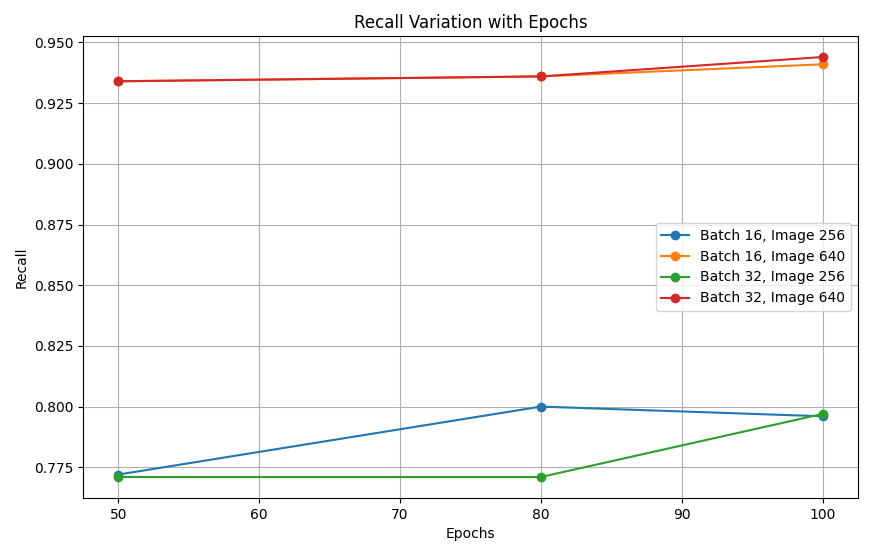
\includegraphics[width=0.6\textwidth]{figs/recall-variation.png} 
    \caption{Recall Variation}
    \label{fig:recall-variation}
\end{figure}

Precision, on the other hand, measures the number of true positive detections out of all positive predictions made 
by the model. While high precision reduces the number of false positives (incorrectly identified weapons), the 
balance between recall and precision is vital. In real-time weapon detection, a slightly lower precision might 
be acceptable if it results in a significantly higher recall. This trade-off ensures that the system prioritizes 
safety by detecting as many weapons as possible, even at the cost of occasional false alarms.

Considering the analysis of the metrics and training times, the optimal configuration for the YOLOv5 
model is 100 epochs, a batch size of 32, and an image size of 640. This 
setup achieves the highest accuracy (0.973), high precision (0.969), and the highest recall (0.944). 
Despite the longer training time, the improved performance justifies the use of a larger batch size and image size.
The high recall ensures that most relevant instances are detected. Simultaneously, the high precision minimizes 
false positives, maintaining the system's reliability and efficiency.

Figure \ref{fig:pr-curve} shows the Precision-Recall Curve for the optimal configuration of the trained model. This curve 
illustrates the trade-off between precision and recall for different classes of objects, being useful for 
understanding the performance of the model in distinguishing between different classes at various threshold levels.

The area under the precision-recall curve (AP) for the weapon class is 0.953. The AP for the knife class is 
significantly higher at 0.991. The mean average precision (mAP) across all classes at an IoU threshold of 
0.5 is 0.972. The curve indicates that the model performs well in detecting knives, followed by 
general weapon detection, with overall high precision and recall values across all classes.

The second image, figure \ref{fig:f1-curve}, shows how the F1 score, which is the harmonic mean of 
precision and recall, varies with the confidence threshold used for classifying detections.
The maximum F1 score for the weapon class is around 0.96. The knife class also achieves a high F1 score, slightly 
above the weapon class. The F1 score for all classes combined reaches 0.96 at a confidence threshold of approximately 
0.392. This curve demonstrates that the model maintains a high F1 score over a range of confidence thresholds, 
indicating that the model is reliable and robust in detecting weapons and knives with balanced precision and recall.

\begin{figure}[h]
    \centering
    \begin{minipage}{0.49\textwidth}
        \centering
        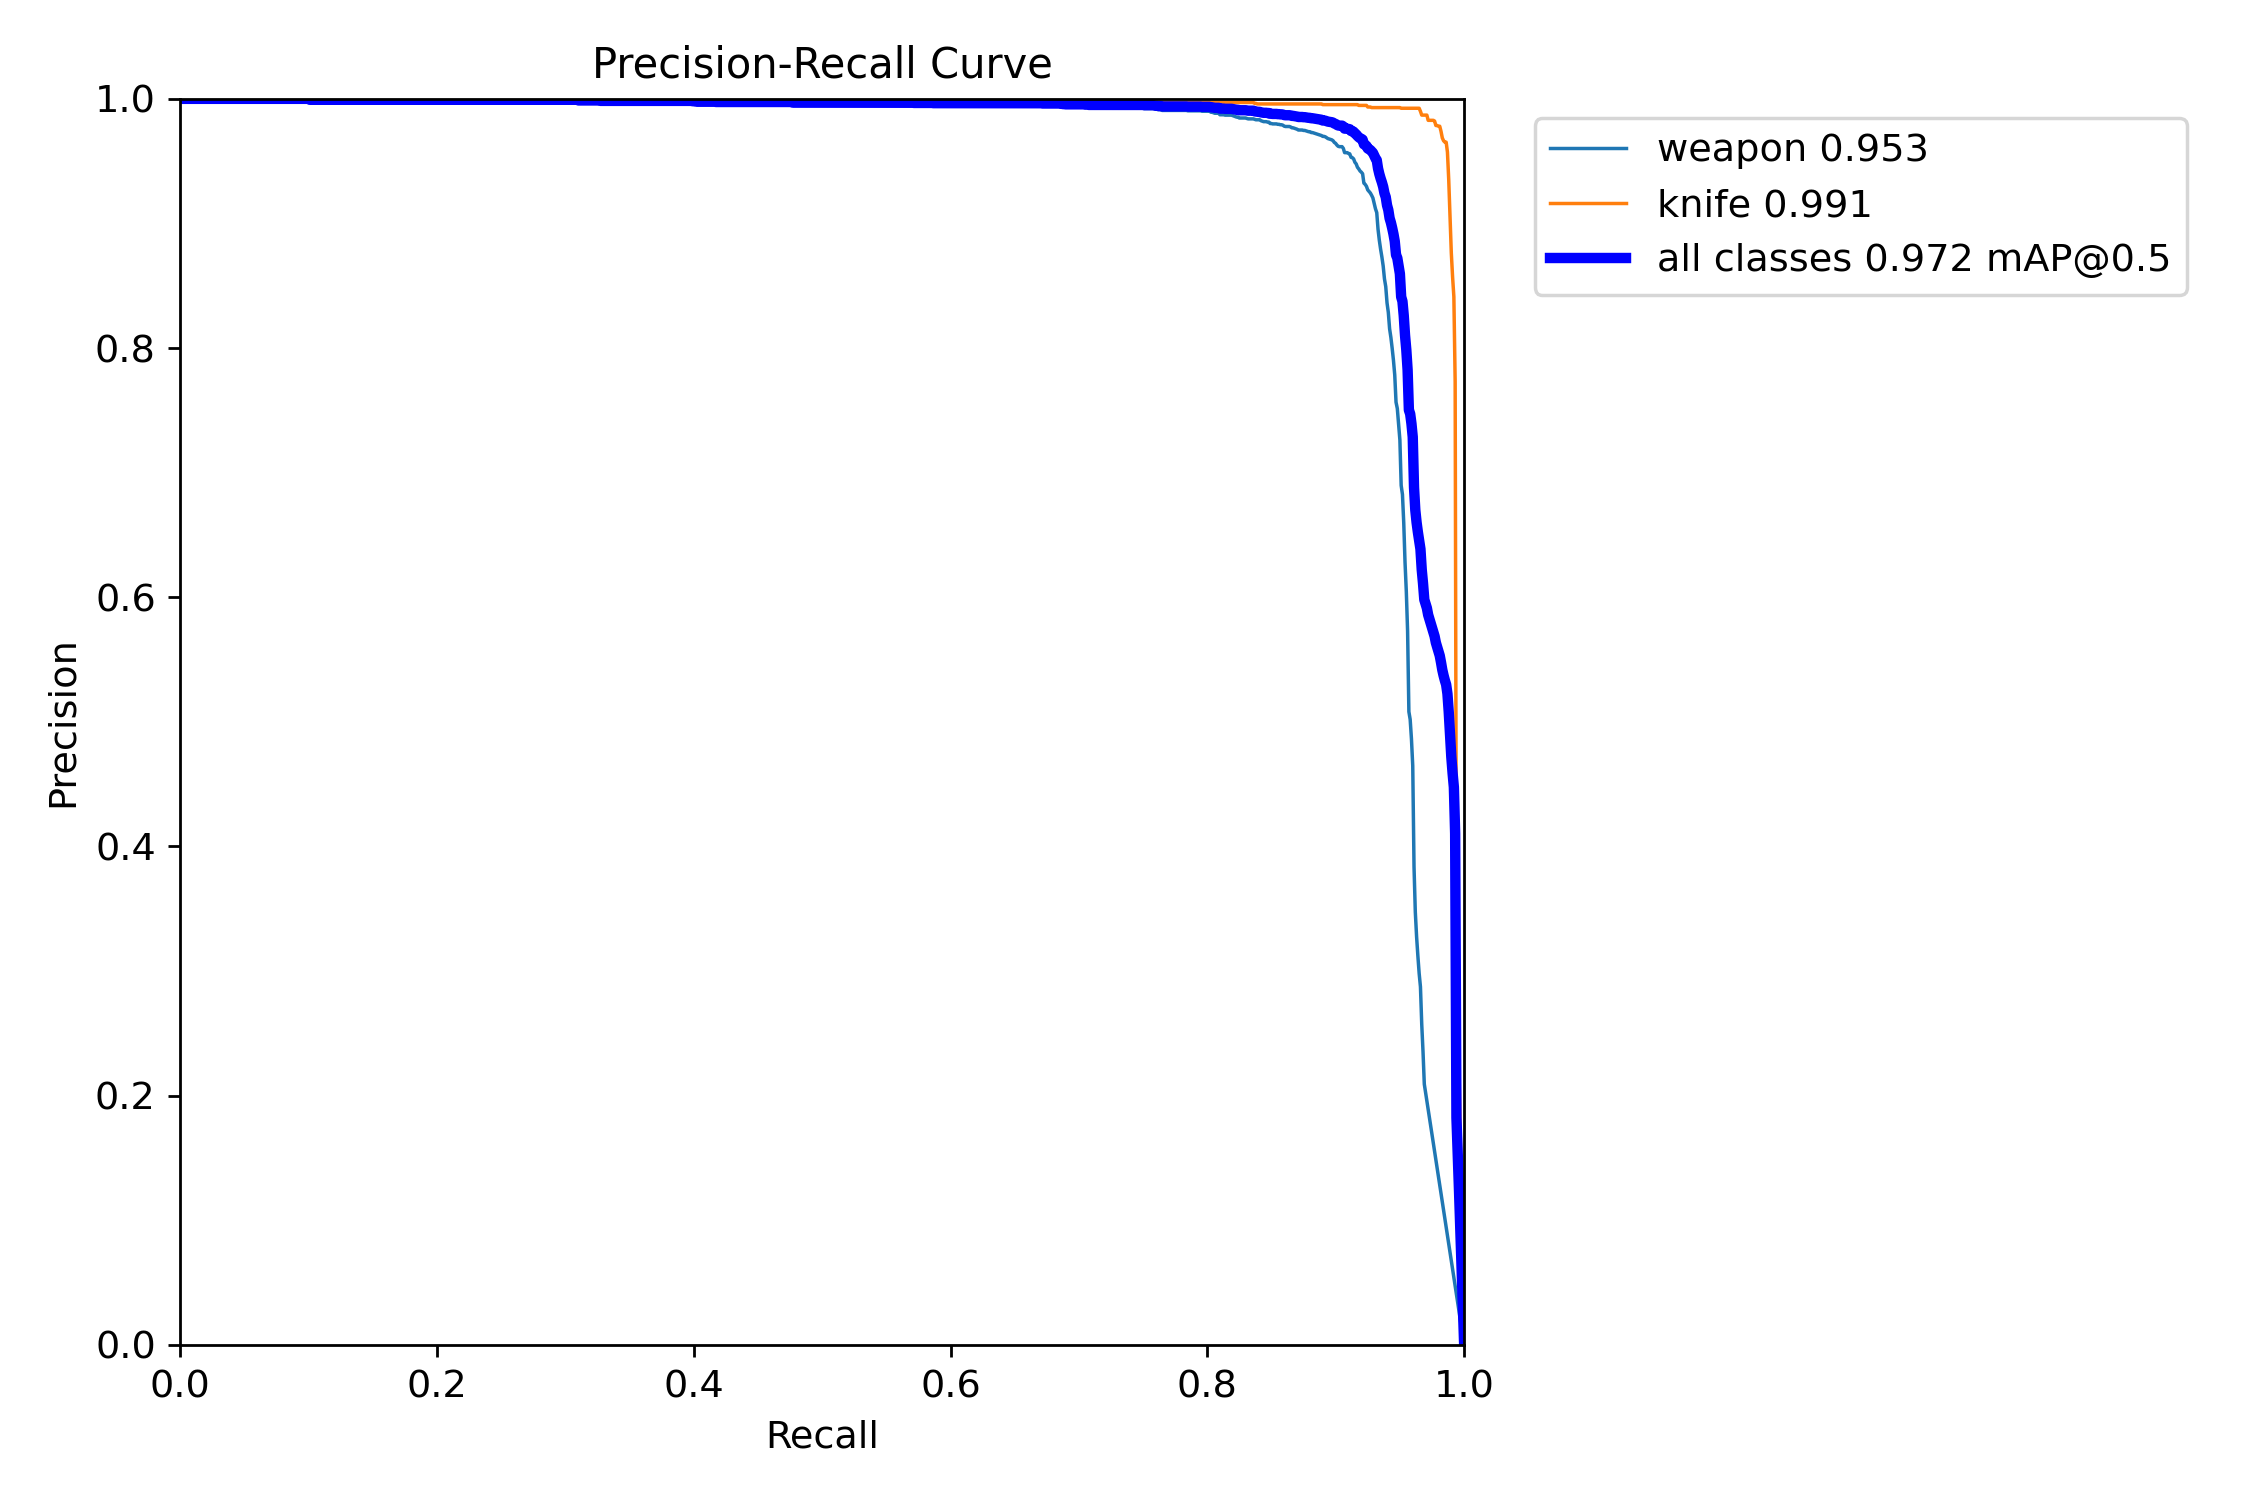
\includegraphics[width=1\linewidth]{figs/PR_curve.png}
        \caption{Precision-Recall Curve}
        \label{fig:pr-curve}
    \end{minipage}\hfill
    \begin{minipage}{0.49\textwidth}
        \centering
        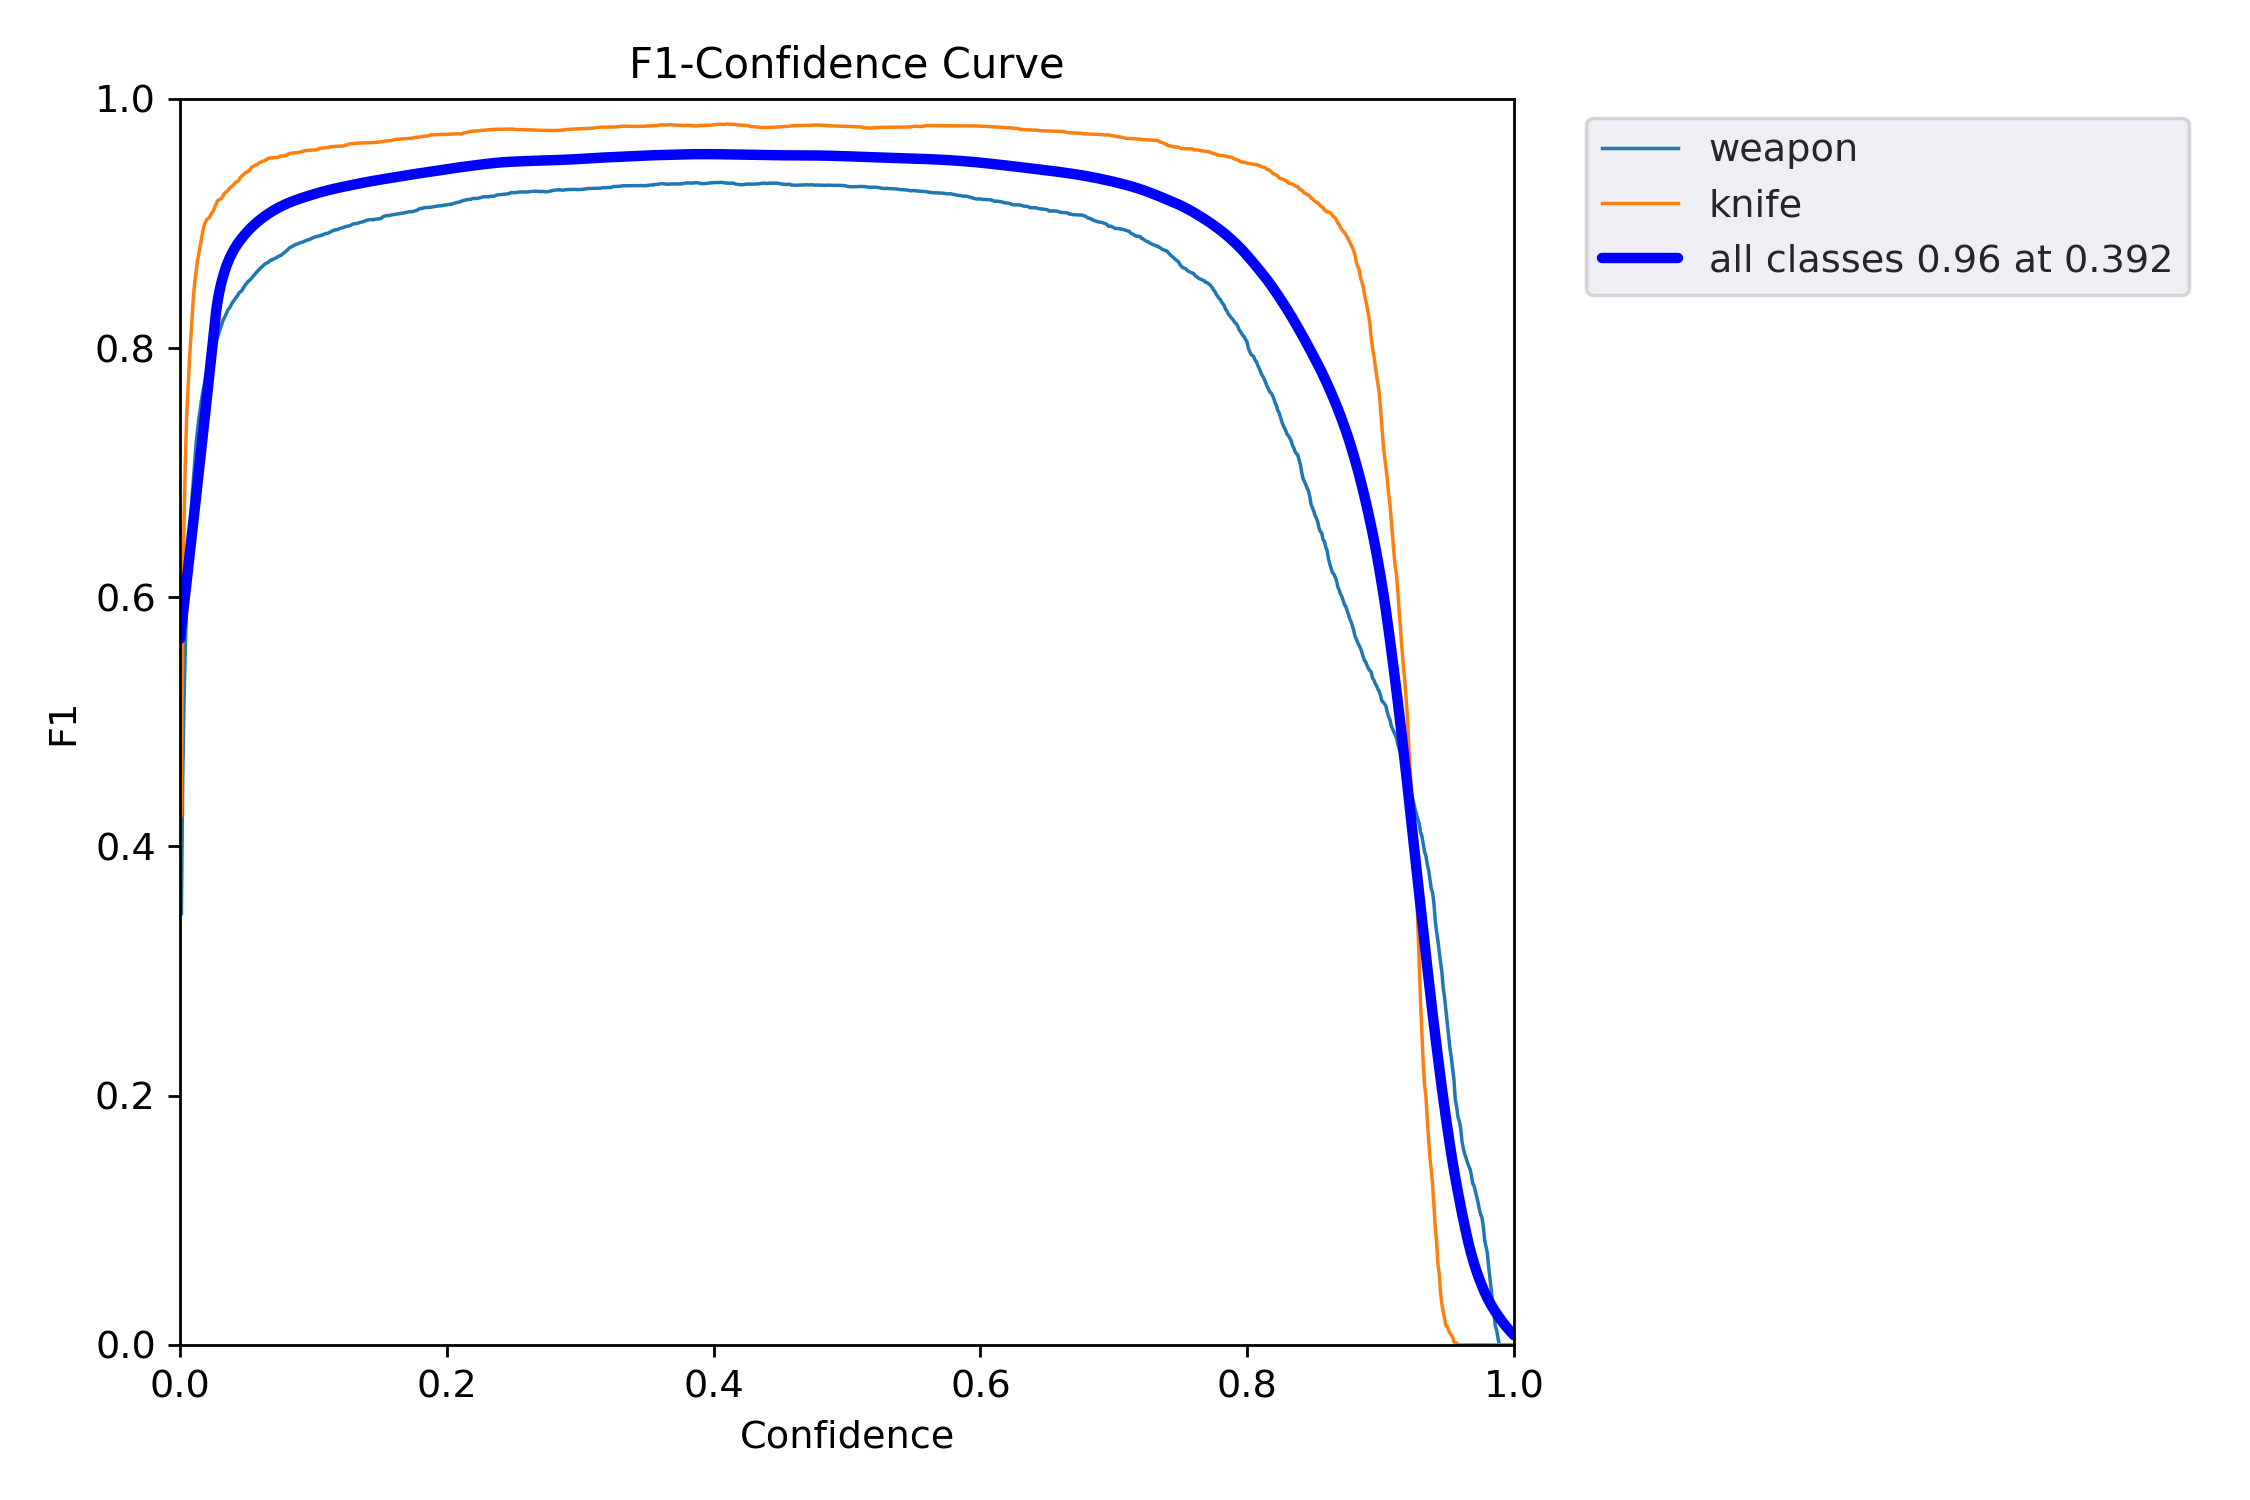
\includegraphics[width=1\linewidth]{figs/F1_curve.png}
        \caption{F1-Confidence Curve}
        \label{fig:f1-curve}
    \end{minipage}
\end{figure}

Figure \ref{fig:conf-matrix} is the Confusion Matrix for a the YOLOv5 model. It has three categories along both 
axes: weapon, knife, and background. The rows represent the 
predicted labels, while the columns represent the true labels. The intensity of the color indicates the number 
of instances, with darker colors representing higher values.

For the weapon class, the model correctly predicted 93\% of the instances, as indicated by the dark blue 
square in the top-left corner. The rest of the weapon instances were misclassified as background, as
shown by the light blue square in the bottom-left corner. Additionally, no instances of weapons were 
misclassified as knives.


For the knife class, the model correctly predicted 98\% of the instances, as shown by the dark blue square 
in the center of the matrix. The remaining 2\% were misclassified as background, 
which is shown by the light blue square in the bottom-center section.

\begin{figure}[h]
    \centering 
    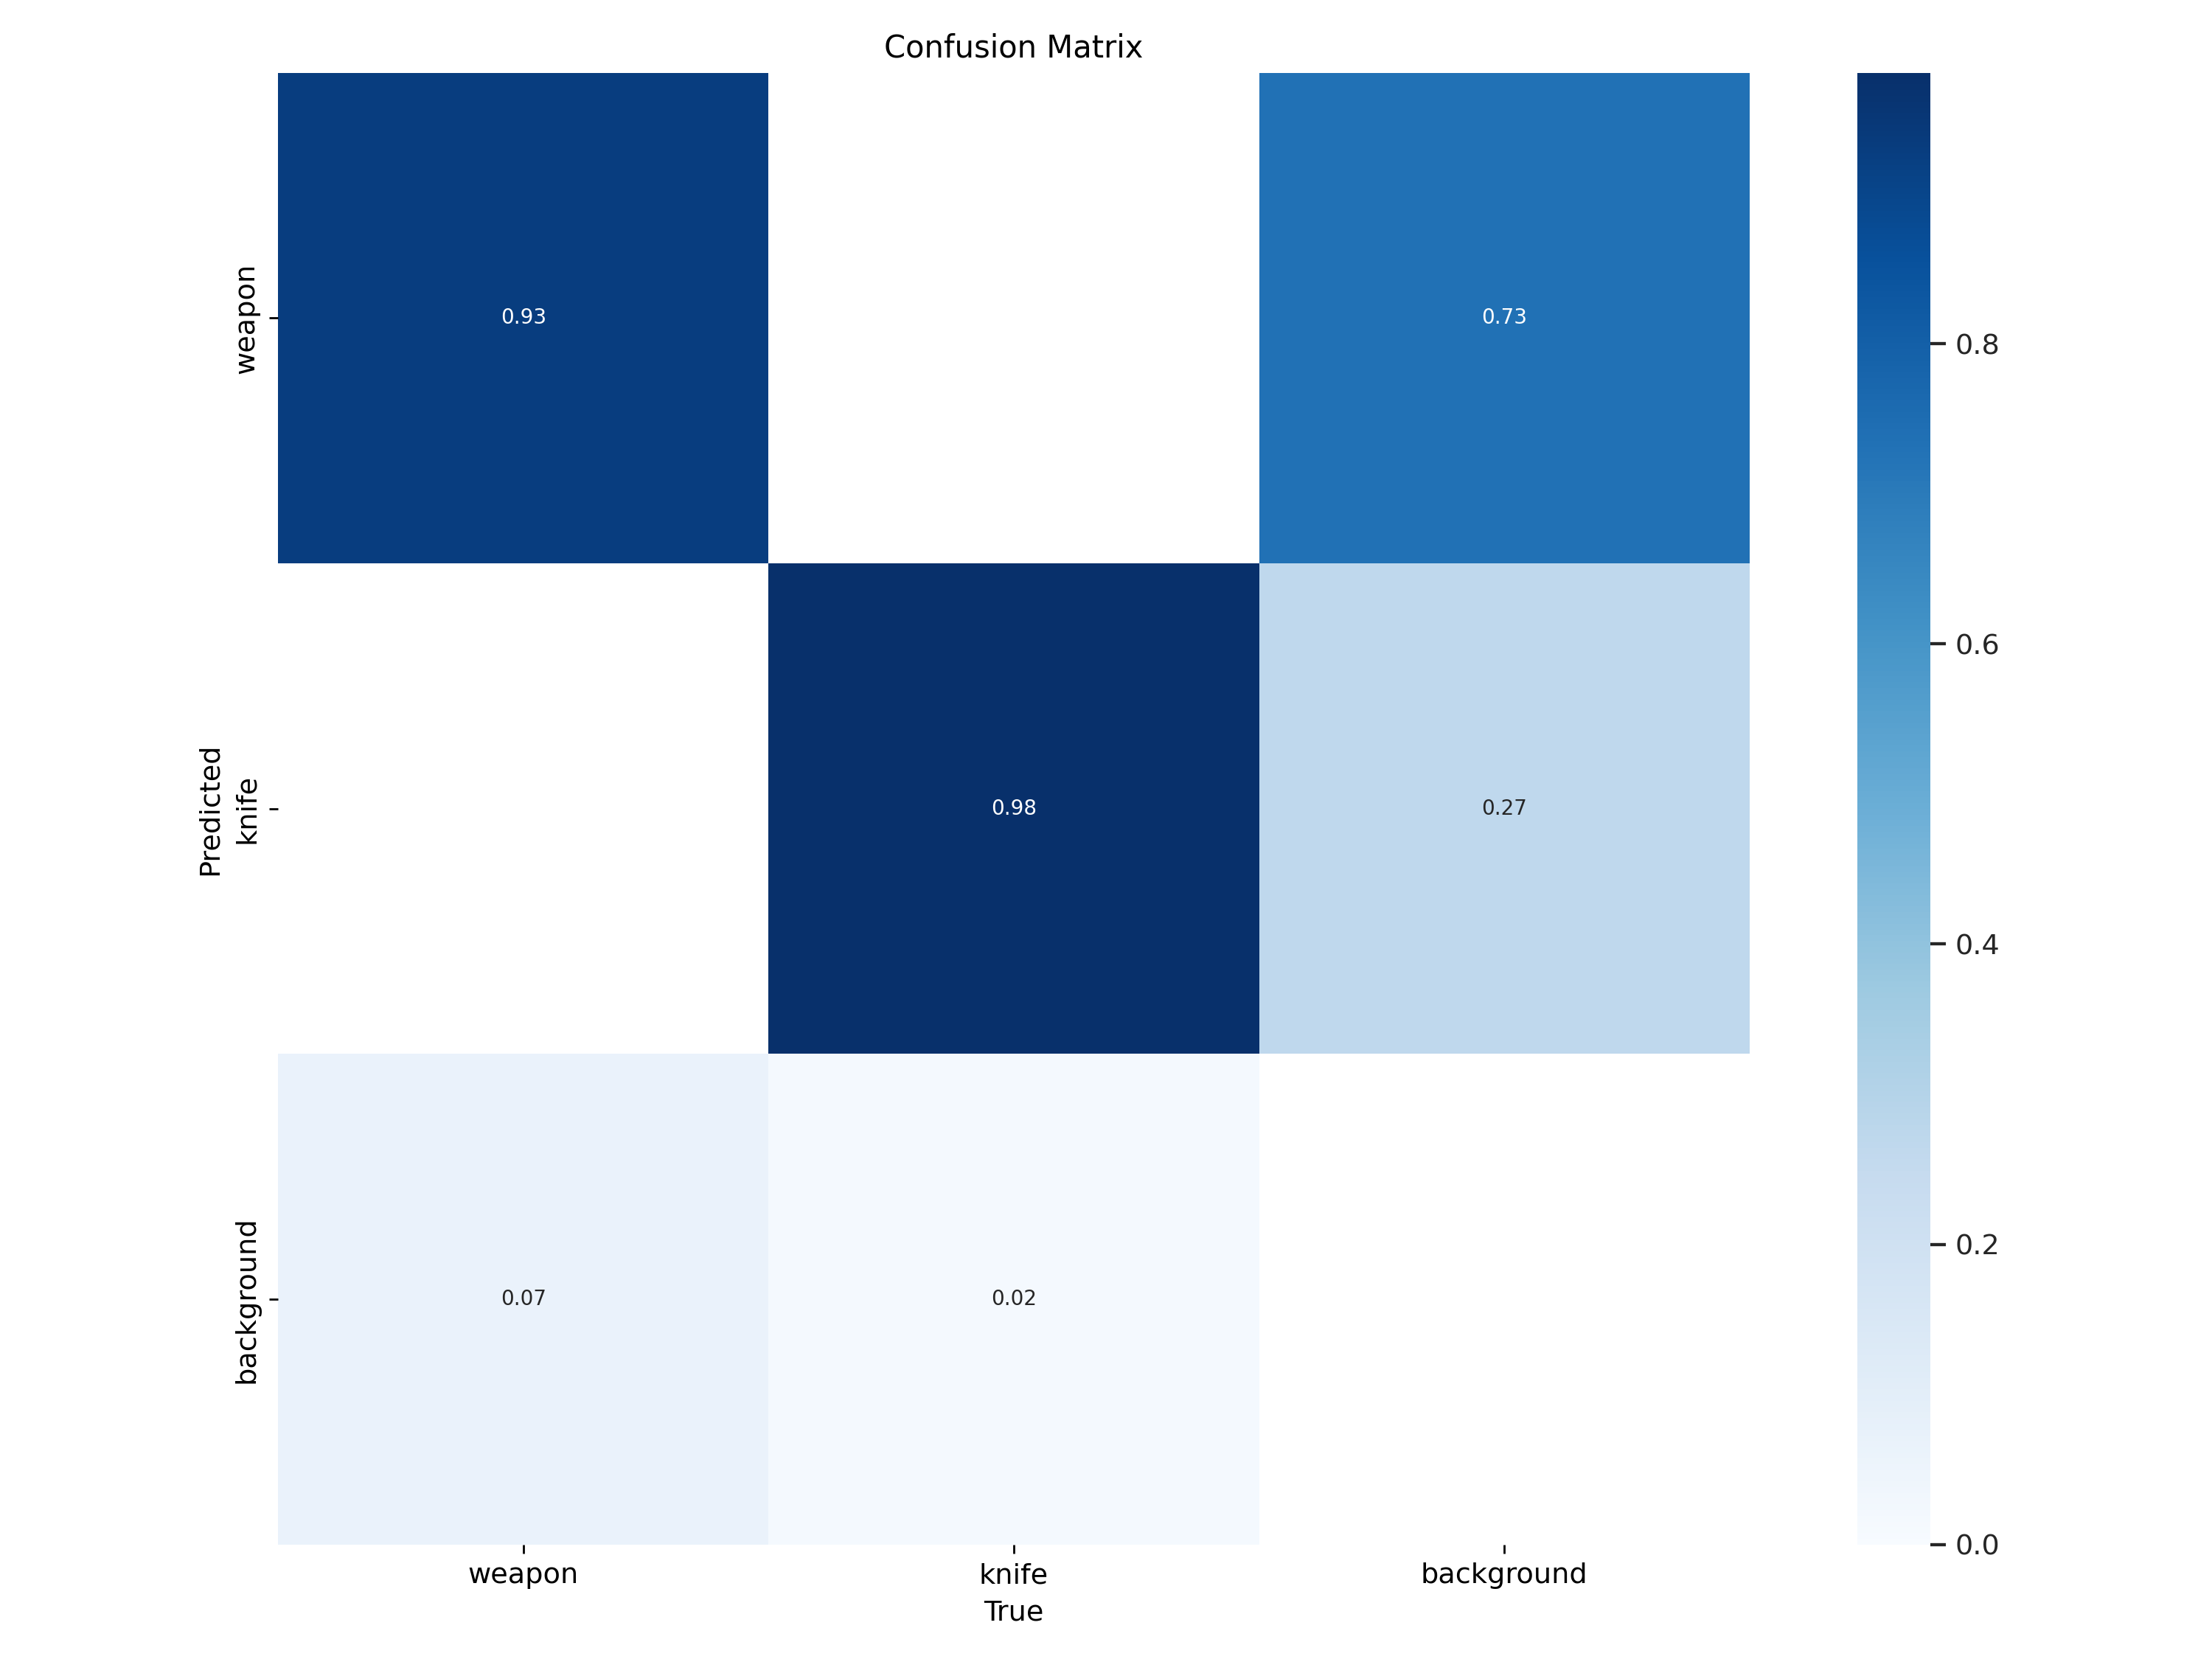
\includegraphics[width=0.7\textwidth]{figs/confusion_matrix.png} 
    \caption{Confusion Matrix}
    \label{fig:conf-matrix}
\end{figure}

\section{Real-World Scenario Testing}
\subsection{Non-Weaponized Scenario Analysis}
The first test scenario is a 9-second video clip featuring a single human subject walking across a room while holding a 
cellphone, as shown in frame \ref{fig:non-weapon-frames1}. The environment is devoid of any weapons. This 
scenario was chosen to evaluate the model's precision in identifying the absence of weapons and ensuring that 
non-threatening objects, such as cellphones, are not incorrectly detected as weapons.

\begin{figure}[h]
    \centering
    \begin{minipage}{0.44\textwidth}
        \centering
        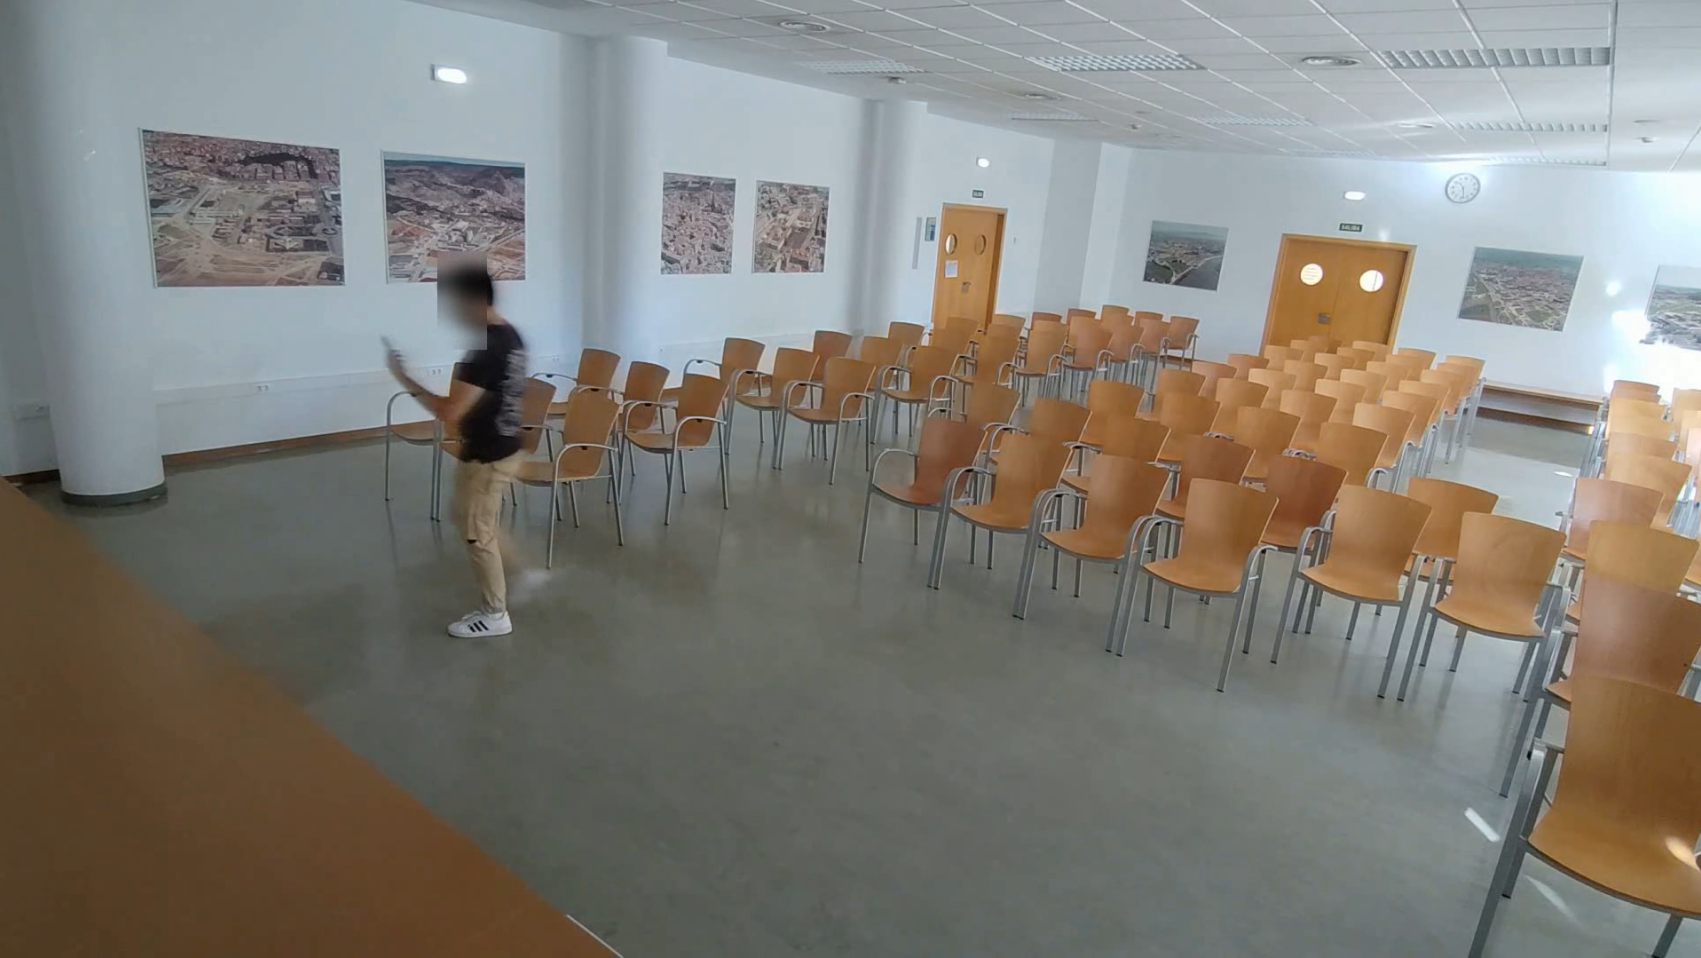
\includegraphics[width=1\linewidth]{figs/non-weapon-frame2.png}
        \caption{Video 1 Frame}
        \label{fig:non-weapon-frames1}
    \end{minipage}\hfill
    \begin{minipage}{0.44\textwidth}
        \centering
        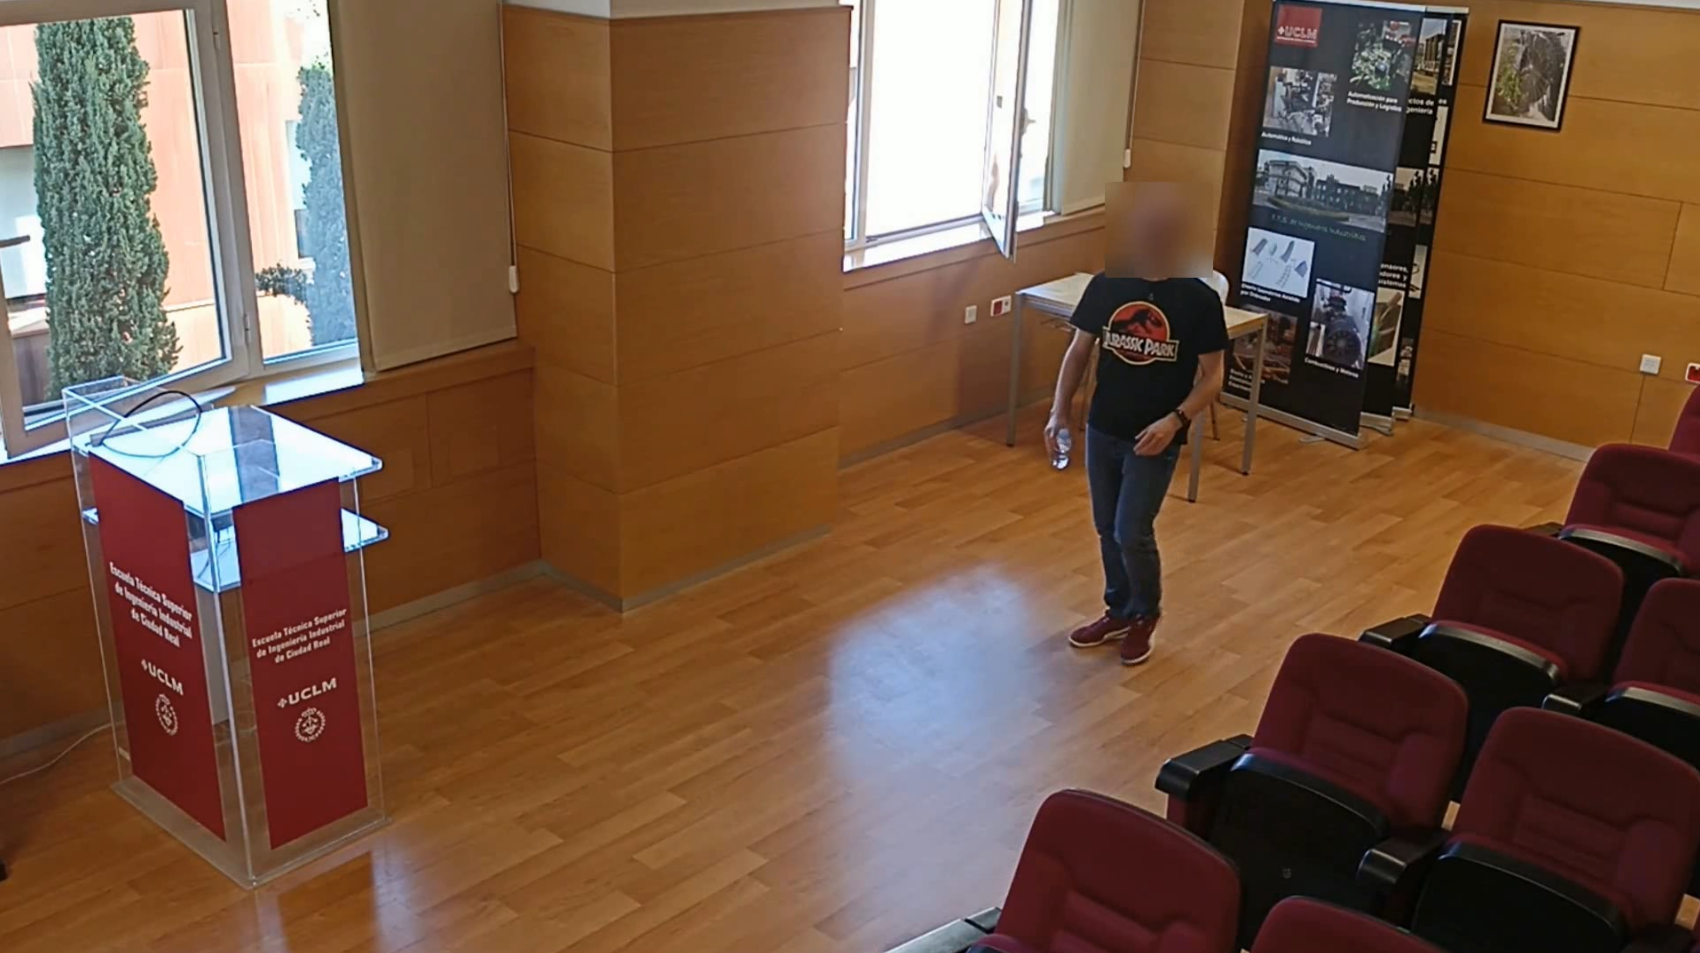
\includegraphics[width=1\linewidth]{figs/non-weapon-frame1.png}
        \caption{Video 2 Frame}
        \label{fig:non-weapon-frames2}
    \end{minipage}
\end{figure}

The object detection model performed optimally in this non-weaponized scenario. Throughout the entire duration of 
the video, the model consistently refrained from flagging the cellphone or any other elements within the room as 
weapons. This result is indicative of the model's accuracy and reliability in distinguishing between actual threats 
and benign objects.

Another video was utilized to further assess the model's performance, examplified in image \ref{fig:non-weapon-frames2}. This test scenario involved a 10-second 
video featuring a human subject holding a water bottle inside a classroom. Similar to the previous scenario, 
the environment was free from any weapons, aiming to verify the model's capability to accurately identify 
non-threatening objects and avoid false positives.

\subsection{Weaponized Environment Detection}
The YOLOv5 model was applied to a 10-second video containing weapons. The video consists of 300 frames, 
approximately 30 frames per second, serving as the test sample.

Figure \ref{fig:frame-annotated} shows a frame annotated by the object detection algorithm, while figure 
\ref{fig:frame-47} shows the same frame without being annotated.

\begin{figure}[h]
    \centering
    \begin{minipage}{0.45\textwidth}
        \centering
        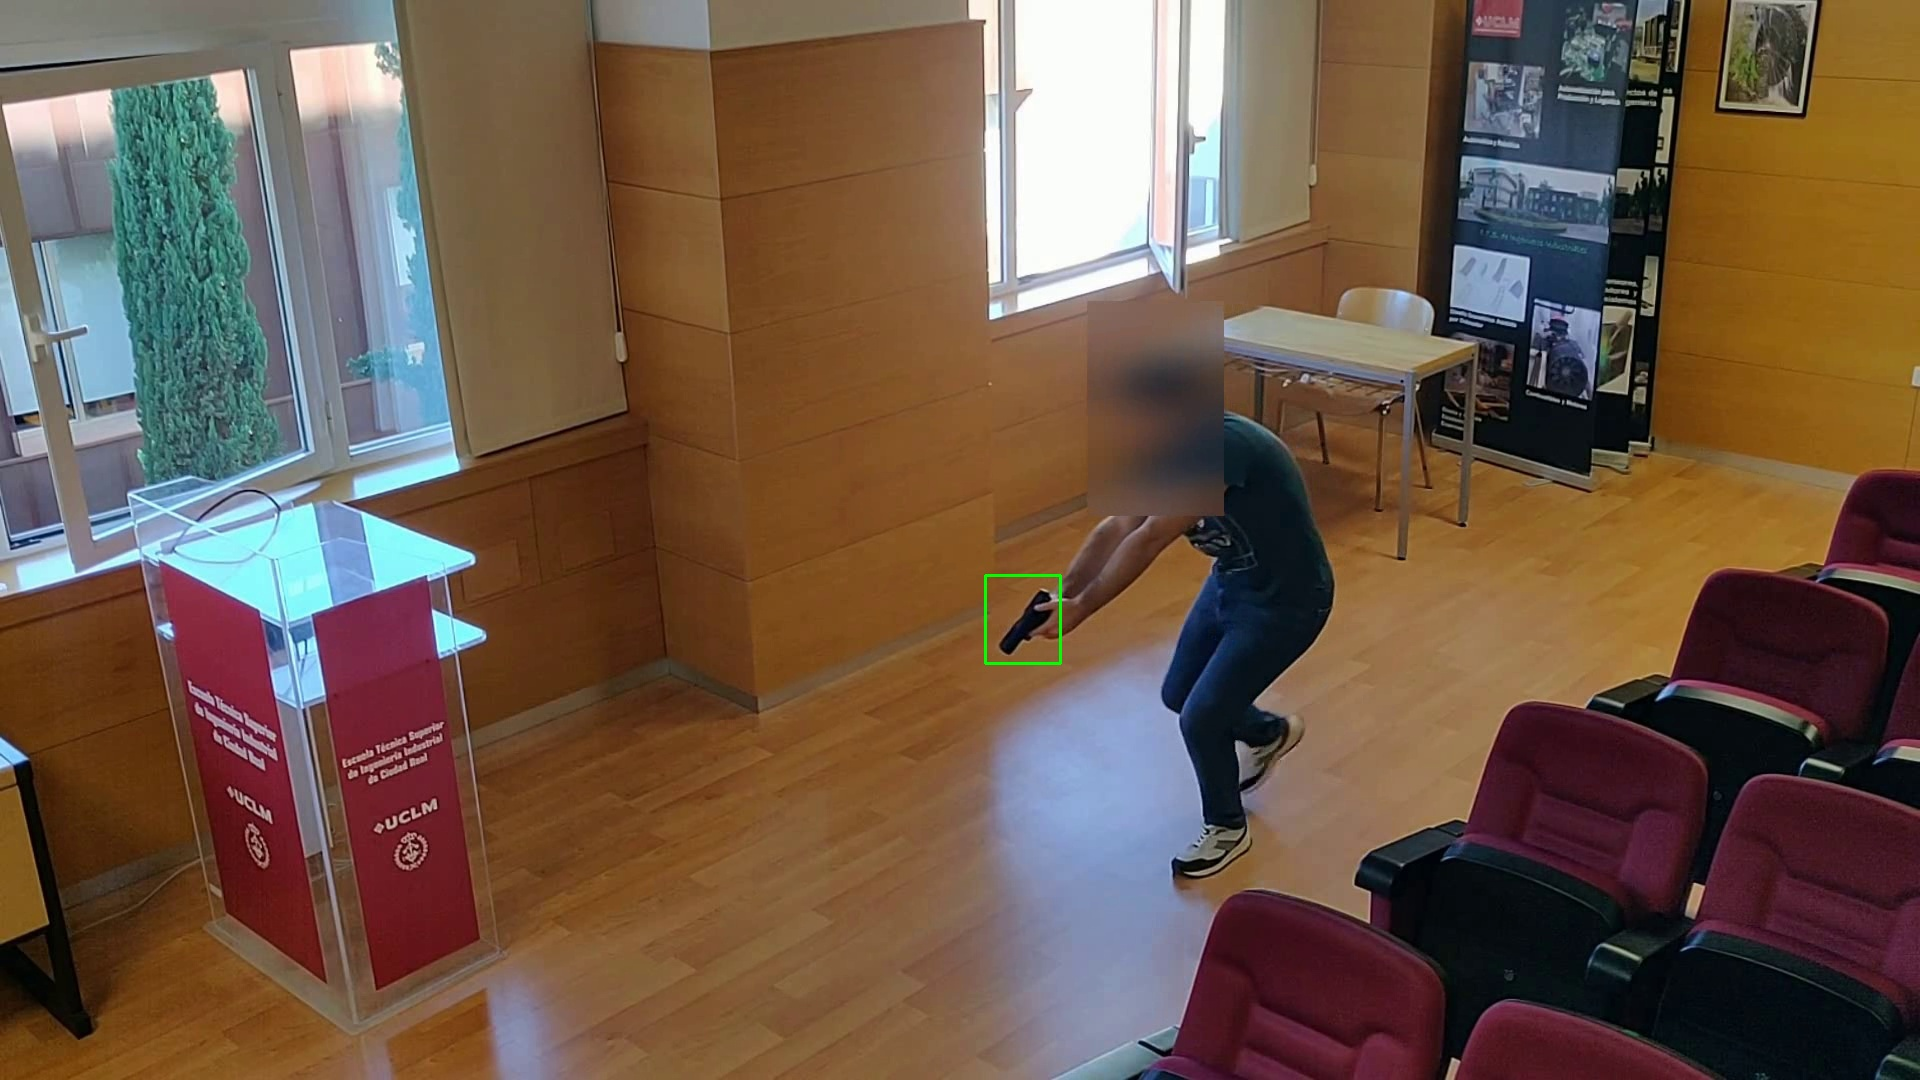
\includegraphics[width=1\linewidth]{figs/annotated_frame_160.jpg}
        \caption{Annotated Frame from Weaponized Environment}
        \label{fig:frame-annotated}
    \end{minipage}\hfill
    \begin{minipage}{0.45\textwidth}
        \centering
        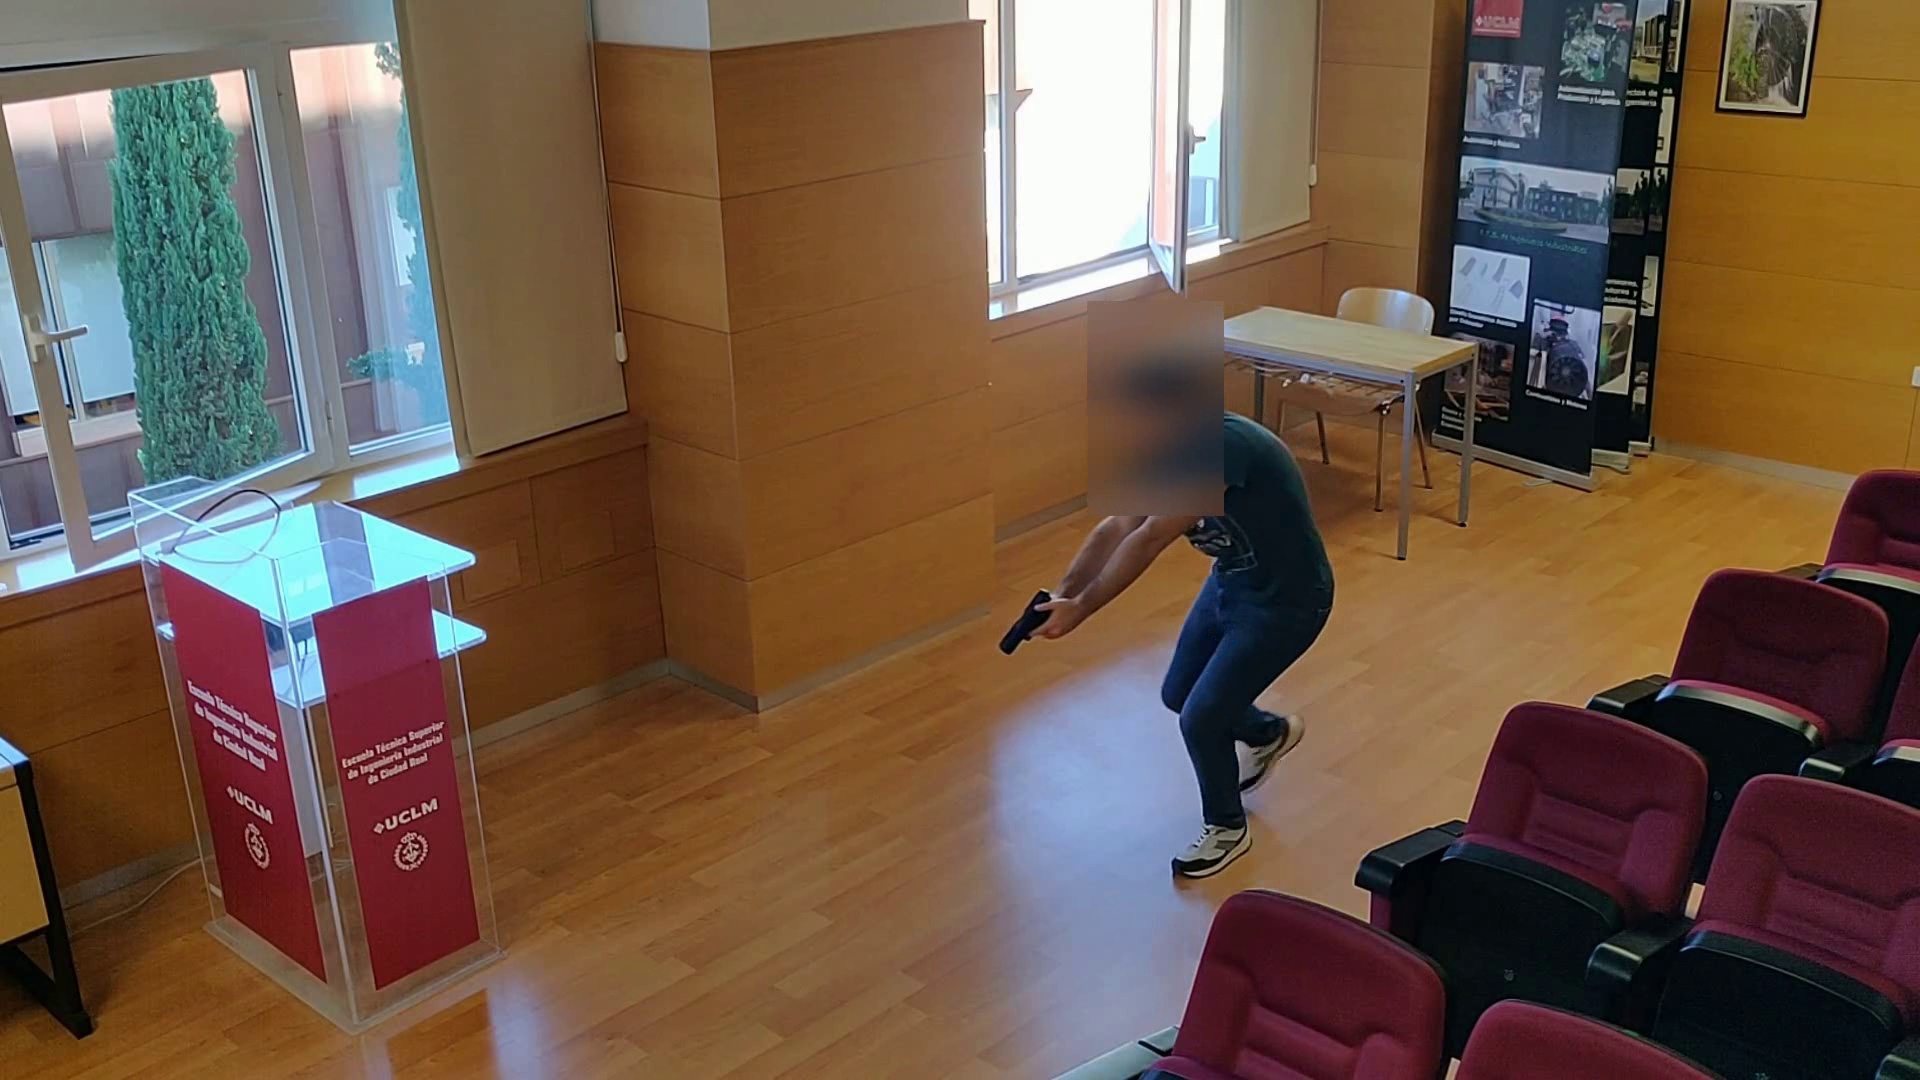
\includegraphics[width=1\linewidth]{figs/frame_160.jpg}
        \caption{Frame From Weaponized Scenario}
        \label{fig:frame-47}
    \end{minipage}
\end{figure}

Out of the 300 frames, 196 frames contained objects of interest, in this case weapons. The YOLOv5 model successfully 
detected 
weapons in 131 of these frames. However, there were 69 frames containing weapons that the model failed to annotate.
Given that 1 second of video has approximately 30 frames and the changes within this short duration are minimal, the 
model demonstrates a reasonable efficiency in identifying objects.

Some frames were not detected because the objects, being dark, were situated against a similarly dark background. 
Additionally, the human face in the video is completely blurred, and in some instances, the weapon 
is obscured behind the blurred face, further complicating detection.

\section{User Experience Evaluation}
To ensure the effectiveness and usability of the application, was organized a presentation and demonstration session 
with the police commissioner from Coimbra.

During this session, all the features and functionalities of the application were presented, showcasing its ability to 
detect weapons and provide immediate alerts. The interface, designed with simplicity, was demonstrated to highlight 
its intuitive navigation and clean layout.

The police commissioner provided valuable feedback on the application. Overall, the feedback was positive, observing that 
the application was intuitive, making it easy for users to navigate and operate without extensive training.

In addition to the positive remarks, the commissioner offered constructive suggestions for further improvements.
One proposed improvement was for the system to be able to upload more than one video at a time.

Following the session, the police commissioner shared the application with police personnel in Coimbra for 
further evaluation and practical testing in real-world scenarios.
\section{Comparative Analysis}
The performance of the pre-trained YOLOv5 model demonstrates superior accuracy compared to the majority of models 
discussed in the related work section. Specifically, the YOLOv5 model consistently achieves higher precision and 
recall rates, indicating its robustness in object detection tasks.

Our solution, in figure \ref{fig:comparative-analysis}, highlighted in red with an accuracy of 0.97, clearly outperforms other models, underscoring its 
effectiveness and reliability in real-time surveillance applications. The best performance among 
the other works is an accuracy of approximately 0.93.

\begin{figure}[h]
    \centering 
    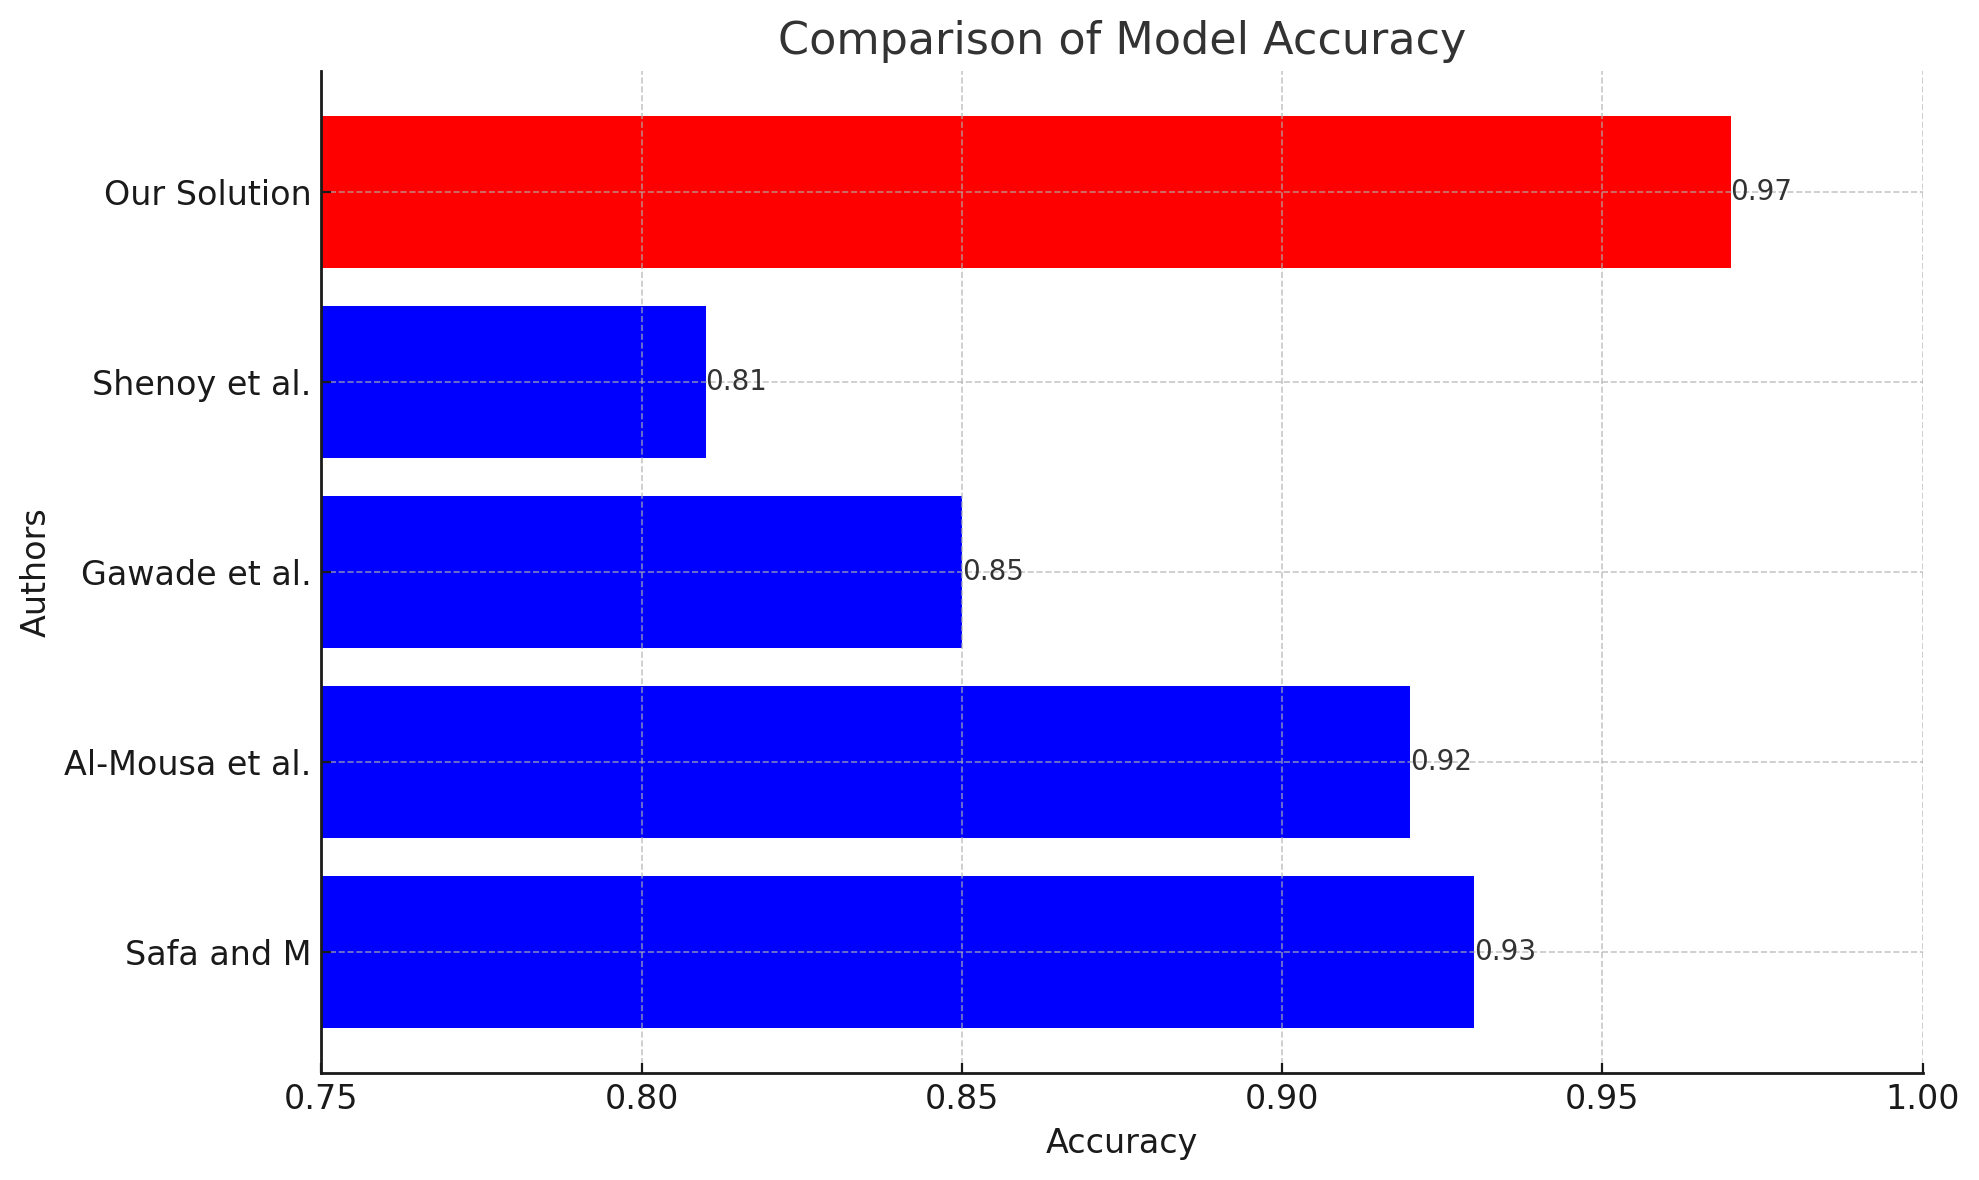
\includegraphics[width=0.6\textwidth]{figs/comparative-analysis.png} 
    \caption{Comparative Analysis with Related Works}
    \label{fig:comparative-analysis}
\end{figure}

This system is a pioneering real-time weapon detection system designed for use by the Coimbra Police Department to 
enhance the safety and efficiency of its officers. It integrates a pre-trained object detection model, 
which has been developed and tested on an extensive and comprehensive dataset, ensuring accurate identification of 
weapons in various scenarios. The model is integrated into a user-friendly web interface, enabling officers 
to access real-time insights and alerts directly from their devices.

As this real-time weapon detection system is a pioneering initiative, there is room for improvement. 
Continuous updates are necessary to enhance its accuracy, reduce false positives, and adapt 
to evolving threats. Feedback from the officers who will be using the system will be crucial in 
identifying areas for enhancement and ensuring the technology meets the practical needs of law enforcement. 
Additionally, expanding the dataset with more diverse and real-world examples can further train the model to 
handle a broader range of scenarios, ultimately improving its robustness and reliability. 